\documentclass[cal1spr16Lectures.tex]{subfiles}
%\AtBeginSubsection{
%	\begin{frame}[allowframebreaks]{}
%	\begin{multicols}{2}
%	\tableofcontents[currentsubsection]
%	\end{multicols}
%	\end{frame}
%	}
	
\begin{document}

%\section[Week 2]{Week 2: 25-29 Jan}

% % %
\subsubsection{\bf Monday 25 January}
\begin{frame}[allowframebreaks]{Mon 25 Jan}
\begin{itemize}\footnotesize
\item \href{http://comp.uark.edu/~ashleykw/Cal1Spring2016/cal1spr16.html}{\alert{\url{comp.uark.edu/~ashleykw/Cal1Spring2016/cal1spr16.html}}} \\
	Course website.  All information is here, including a link to MLP, lecture slides, administrative information, etc.  You should have already seen the 
	\href{http://comp.uark.edu/~ashleykw/Cal1Spring2016/syllabusCal1Spring2016.pdf}{\alert{\textbf{syllabus}}}
	by now.
\item MyLabsPlus (MLP) has the graded homework.   Solutions to Quizzes and Drill exercises will be posted there, under ``Menu $\to$ Course Tools $\to$ Document Sharing".  
%
\framebreak 
\item Lecture slides are available on the course website.  I'll try to have the week's slides posted in advance but the individual lectures might not be posted until right before class.  \textbf{Don't try to take notes from the slides.}  Instead, print out the slides beforehand or else follow along on your tablet/phone/laptop.  You should, however, take notes when we do exercises during lecture.% (which is frequent).  We will always review those solutions on the document camera.  Document camera notes are reserved only for those who attended lecture that day.  :p

\alert{Suggestion:} When printing the slides, put more than one slide per page and print double-sided.  
%
\framebreak
\item For old Calculus materials, see the parent page \url{comp.uark.edu/~ashleykw} and look for links under ``Previous Semesters".  
%
%\framebreak
\item GET YOUR CLICKER	
\item Note: There is no Blackboard for this course.
\item Stay on top of the MLP!  First deadline is coming up.  Don't wait till the last minute.
\item MLP issues...
\item Quiz 1 is due in drill \alert{tomorrow}.  See MLP for a copy.
\end{itemize}
\end{frame}

% % %
\subsubsection{Additional (Algebra) Techniques}
\begin{frame}{\small Additional (Algebra) Techniques}\footnotesize
When direct substitution (a.k.a. plugging in $a$) fails try using algebra:

\vspace{0.25pc}
\begin{itemize}
\item Factor and see if the denominator cancels out.
\begin{ex} $\lim_{t \to 2} \frac{3t^2-7t+2}{2-t}$ \end{ex}

\vspace{0.25pc}
\item Look for a common denominator.
\begin{ex} $\lim_{h \to 0} \frac{ \frac{1}{5+h}-\frac{1}{5} }{h}$ \end{ex}
\end{itemize}
\end{frame}

% % % 
\begin{frame}
\begin{exe}
Evaluate $\lim_{s\to 3}\frac{\sqrt{3s+16}-5}{s-3}$.
\end{exe}
\end{frame}

% % %
\subsubsection{Another Technique: Squeeze Theorem}
\begin{frame}{\small Another Technique: Squeeze Theorem}
This method for evaluating limits uses the relationship of functions with each other.

\begin{thm}[Squeeze Theorem]\footnotesize  Assume $f(x)\leq g(x)\leq h(x)$ for all values of $x$ near $a$, except possibly at $a$, and suppose
\[\lim_{x \to a}f(x)=\lim_{x \to a} h(x)=L.\] 
Then since $g$ is always between $f$ and $h$ for $x$-values close enough to $a$, we must have 
\[\lim_{x \to a} g(x)=L.\] \end{thm}
\end{frame}

% % %
\begin{frame}
\begin{ex} \begin{itemize}
\item[(a)]Draw a graph of the inequality 
\[-|x| \leq x^2 \ln{(x^2)} \leq |x|.\]

\vspace{0.5pc}
\item[(b)] Compute $\lim_{x \to 0} x^2 \ln{(x^2)}.$
\end{itemize}
\end{ex}
\end{frame}

% % %
\subsubsection{Book Problems}
\begin{frame}
\begin{block}{2.3 Book Problems} 12-30 (every 3rd problem), 33, 39-51 (odds), 55, 57, 61-67 (odds) \end{block}
%\begin{itemize}
%\item 
In general, review your algebra techniques, since they can save you some headache.
%\end{itemize}
\end{frame}

% % %
\subsection[2.4 Infinite Limits]{\S 2.4 Infinite Limits}
% % %

% % %
\begin{frame}{\S 2.4 Infinite Limits}
We have examined a number of laws and methods to evaluate limits.  
\begin{que}
Consider the following limit: 
\[
\lim_{x\to 0}\frac{1}{x}
\]
How would you evaluate this limit?
\end{que}
\end{frame}

% % %
\begin{frame}{}\footnotesize
In the next two sections, we examine limit scenarios involving infinity.  The two situations are:
\begin{itemize}
\item {\bf Infinite limits:}  as $x$ (i.e., the independent variable) approaches a finite number, $y$ (i.e., the dependent variable) becomes arbitrarily large or small

\vspace{0.5pc}
\hspace{50pt}looks like: $\displaystyle\lim_{x\to\text{number}}f(x)=\pm\infty$
\item {\bf Limits at infinity:} as $x$ approaches an arbitrarily large or small number, $y$ approaches a finite number

\vspace{0.5pc}
\hspace{50pt}looks like: $\displaystyle\lim_{x\to\pm\infty}f(x)=\text{number}$
\end{itemize}
\end{frame}

% % %
\subsubsection{Definition of Infinite Limits}
\begin{frame}{\small Definition of Infinite Limits}
\begin{dfn}[positively infinite limit] Suppose $f$ is defined for all $x$ near $a$.  If $f(x)$ grows arbitrarily large for all $x$ sufficiently close (but not equal) to $a$, we write
\[\lim_{x \to a} f(x) = \infty\]
and say {\bf the limit of $f(x)$ as $x$ approaches $a$ is infinity}. \end{dfn}
\end{frame}

% % %
\begin{frame}
\begin{center}
\noindent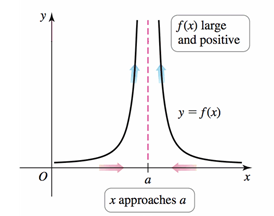
\includegraphics[scale=1]{pictures/Fig2_24a}
\end{center}
\end{frame}

% % %
\begin{frame}
\begin{dfn}[negatively infinite limit] Suppose $f$ is defined for all $x$ near $a$.  If $f(x)$ is negative and grows arbitrarily large in magnitude for all $x$ sufficiently close (but not equal) to $a$, we write
\[\lim_{x \to a} f(x) = -\infty\]
and say {\bf the limit of $f(x)$ as $x$ approaches $a$ is negative infinity}. \end{dfn}
\end{frame}

% % %
\begin{frame}
\begin{center}
\noindent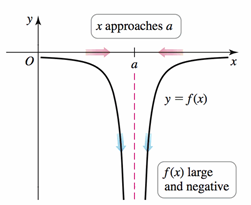
\includegraphics[scale=1]{pictures/Fig2_24b} 
\end{center}
\end{frame}

% % %
\begin{frame}\footnotesize
The definitions work for one-sided limits, too.  

\vspace{1.5pc}
\begin{exe} Using a graph and a table of values, given $f(x)=\displaystyle\frac{1}{x^2-x}$, determine:
\begin{itemize}
\item[(a)\;] $\displaystyle\lim_{x \to 0^+} f(x)$
\item[(b)\;] $\displaystyle\lim_{x \to 0^-} f(x)$
\item[(c)\;] $\displaystyle\lim_{x \to 1^+} f(x)$
\item[(d)\;] $\displaystyle\lim_{x \to 1^-} f(x)$ 
\end{itemize}
\end{exe}
\end{frame}



\end{document}